\documentclass[10pt]{beamer}
\usepackage[brazilian]{babel}
\usepackage[utf8]{inputenc}
\usepackage{kpfonts} % load a font with all the characters
\usepackage[T1]{fontenc}
\usetheme[left]{AAUsidebar}

\usepackage{helvet}

\newcommand{\chref}[2]{\href{#1}{{\usebeamercolor[bg]{AAUsidebar}#2}}%
}

\title[Medidas de Centralidade]{\textbf{MEDIDAS DE CENTRALIDADE}}

\subtitle{}  

\date{\today}

\author[Silvana,  Rodrigo, Guilherme,  Watson] 
{
  Silvana Trindade\\
  Rodrigo Levinski\\
  Guilherme Bizzani\\
  Watson Vieira Costa Junior\\
}

\institute[
  {
\includegraphics[scale=0.1]{AAUgraphics/Logo}}\\ ]
{
  Ciência da Computação\\
  Universidade Federal da Fronteira Sul\\
}

\pgfdeclareimage[height=3cm]{titlepagelogo}{AAUgraphics/Logo} 
\titlegraphic{
  \pgfuseimage{titlepagelogo}
}


\begin{document}
{\aauwavesbg
\begin{frame}[plain,noframenumbering] 
  \titlepage
\end{frame}}
\begin{frame}{Sumário}{Sumário}
\tableofcontents
\end{frame}


\section{Medidas de Centralidade}

\begin{frame}{Medidas de Centralidade}{Centralidade}
\begin{itemize}
\item Que nós são importantes dentro de uma rede?
\item Quais são importantes estruturalmente e relevantes para o fluxo de informação na rede?
\item Intuitivamente, os vértices mais centrais são aqueles que a partir dos quais podemos atingir qualquer outro com mais facilidade ou rapidez.
\end{itemize}
\end{frame}

\section{Rede Sobrevivente}
\begin{frame}{Rede Sobrevivente}{Rede Sobrevivente}
\begin{figure}[htp]
     \centering
     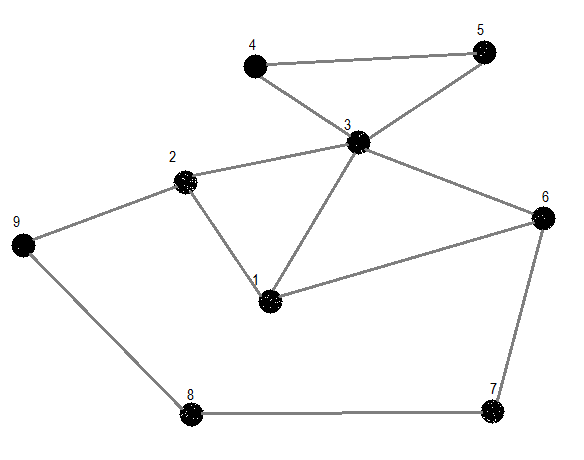
\includegraphics[scale=0.4]{vianet.png}
     \caption{VIA Network.}
      \label{fig:vianet}
\end{figure}
\end{frame}
\section{Centralidade de Grau}
\begin{frame}{Centralidade de Grau}{Centralidade de Grau}
\begin{itemize}
\item \textit{Definição:} De modo mais simples, dizemos que conforme o número de arestas em um vértice mais central, maior é o seu valor como um canal de informações.
\begin{equation}
d_k= \sum_{j=1}^n a_{kj},
\end{equation}
onde o grau do vértice $d_k$ constituído pela soma da matriz de adjacências $a_{kj}$
\begin{equation}
C'_D(v_k) = \frac{d_k}{n-1}.
\end{equation}
Na centralidade relativa é utilizada a proporção do grau em relação ao tamanho do grafo.
\item Exemplo utilizando VIA Network.
\end{itemize}
\end{frame}

\section{Centralidade de Intermediação}
\begin{frame}{Centralidade de Intermediação}{Intermediação}
\begin{itemize}
\item $c_B$ indica o potencial de um vértice no grafo.
\item $v_k$ controla o fluxo de informação entre pares de vértices.
\item Grafos conexos e desconexos (FREEMAN,1977).
\item Geodésicas: caminho de tamanho mínimo entre um nó origem $s$ e destino $t$.
\item Betweenness Centrality: \begin{equation} 
		c_B(v_k)=\sum_{1\leqslant i < j \leqslant n}^{n} b_{ij}(v_k) 
		\end{equation}
\end{itemize}
\end{frame}

\begin{frame}{Centralidade de Intermediação}{Intermediação}
\begin{itemize}
\item $b_{ij}=\frac{g_{ij}(v_k)}{g_{ij}}$, onde $g_{ij}$ corresponde ao número de geodésicas entre $s$ e $t$ e $g_{ij}(v_k)$ o número de geodésicas que possuem o vértice $v_k$ em seu caminho.
\item Limite considerando um grafo com mais de três vértices
\begin{equation}
0 \leqslant c_B(v_k) \leqslant\frac{N^2-3N+2}{2}
\end{equation}
\item Importância da medida
\item Exemplo utilizando a rede VIA Network.
\end{itemize}
\end{frame}

\section{Centralidade de Proximidade}
\begin{frame}{Centralidade de Proximidade}{Proximidade}
\begin{itemize}
\item \textit{Definição:} Em vários contextos, mais importante que ter muitas conexões é não estar longe demais dos demais nós. Proposta por Sabidussi em 1966, a centralidade de proximidade é baseada na soma das distâncias de um vértice em relação aos demais vértices do grafo.

\begin{equation}
C_c(v_k) = \frac{1}{\sum_{j = 1}^n dist(v_j,v_k)} 
\end{equation}
\item Exemplo utilizando VIA Network.
\end{itemize}
\end{frame}


\section{Centralidade de Eficiência}
\begin{frame}{Centralidade de Eficiência}{Eficiência}
\textit{Definição: }
\begin{itemize}
\item Determinar um local de modo que minimize o tempo máximo de viagem entre o mesmo e todas as demais localizações.
\item HAGE e HARARY, em 1995, propuseram uma medida chamada centralidade de eficiência baseada  no  conceito  de  excentricidade  de  um  vértice.
\item Esta medida indica que um vértice é mais eficiente quanto menor for a sua excentricidade.
\item \begin{equation}
C_{eff}(v_k)= \frac{1}{e(v_k)},
\end{equation}
onde $e(v_k)$ = $max\{dist(v_j,v_k):v \in V\}$
\end{itemize}
\end{frame}

\section{Centralidade de Excentricidade}
\begin{frame}{Centralidade de Excentricidade }{Excentricidade}
\begin{itemize}
\item A excentricidade de um nó traduz a ideia do quanto um nó $s$ está distante dos demais nós em um grafo $G$ (BORBA,2013).
\item A excentricidade de um vértice $s$, denotada por $e(s)$, é a máxima das distâncias $dist(s,t)$, isto é, para todo $t$ pertencente a $G$, $e(s)= max\{dist(s,t)\}$.
\item Ou seja, denomina-se excentricidade de um vértice $s \in V$ ao valor da distância máxima entre $s$ e $t$, para todo $t \in V$.
\end{itemize}
\end{frame}

\section{Mais um Exemplo}
\begin{frame}{Mais um Exemplo}{Exemplo}
\begin{figure}[htp]
     \centering
     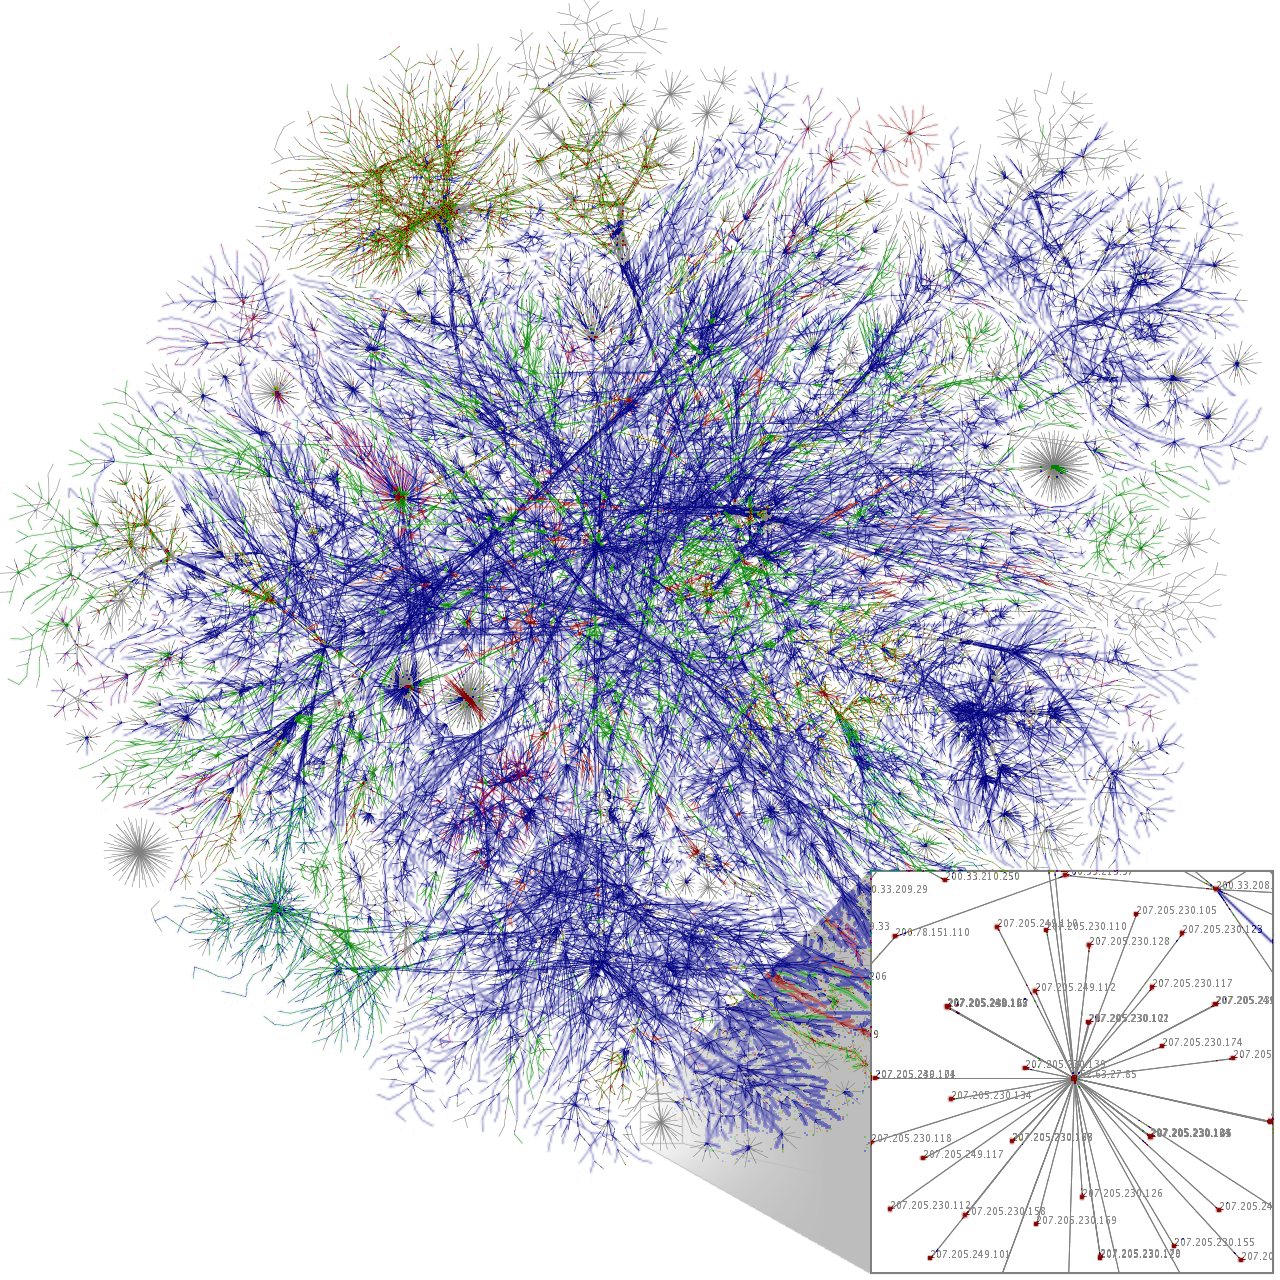
\includegraphics[scale=0.18]{Internet_map_1024_-_transparent.png}
     %\caption{\url{http://puzzle.ics.hut.fi/ICS-A1120/material/_images/Internet_map_1024_-_transparent.png}.}
      \label{fig:vianet}
\end{figure}
\end{frame}

\section{Conclusão}
\begin{frame}{Conclusão}{Conclusão}
"O grau é uma medida da influência direta que um vértice tem em relação a seus contatos, a 
proximidade está relacionada com o tempo que uma informação leva para ser compartilhada por todos os vértices na rede, e a intermediação de um vértice pode ser considerada como o controle da comunicação entre todos os demais pares de vértices da rede." (FREITAS,2010)
\end{frame}
{\aauwavesbg
\begin{frame}[plain,noframenumbering]
  \finalpage{Agradecemos sua atenção!}
\end{frame}}

\end{document}
